\documentclass{article}

% if you need to pass options to natbib, use, e.g.:
% \PassOptionsToPackage{numbers, compress}{natbib}
% before loading nips_2016
%
% to avoid loading the natbib package, add option nonatbib:
% \usepackage[nonatbib]{nips_2016}

\usepackage[final]{nips_2016}

% to compile a camera-ready version, add the [final] option, e.g.:
% \usepackage[final]{nips_2016}
\usepackage[utf8]{inputenc} % allow utf-8 input
\usepackage[T1]{fontenc}    % use 8-bit T1 fonts
\usepackage{hyperref}       % hyperlinks
\usepackage{url}            % simple URL typesetting
\usepackage{booktabs}       % professional-quality tables
\usepackage{amsfonts}       % blackboard math symbols
\usepackage{nicefrac}       % compact symbols for 1/2, etc.
\usepackage{microtype}      % microtypography
\usepackage{graphicx}
\usepackage{float}

\title{Unsupervised Cross-domain Image Generation with Generative Adversarial Network}

% The \author macro works with any number of authors. There are two
% commands used to separate the names and addresses of multiple
% authors: \And and \AND.
%
% Using \And between authors leaves it to LaTeX to determine where to
% break the lines. Using \AND forces a line break at that point. So,
% if LaTeX puts 3 of 4 authors names on the first line, and the last
% on the second line, try using \AND instead of \And before the third
% author name.

\author{
	Liwei Cai 2014011255\\
	Department Electronic Engineering\\
	Tsinghua University\\
	\texttt{clw14@mails.tsinghua.edu.cn} \\
	%% examples of more authors
	\And
	Kaidi Cao 2014012282\\
	Department Electronic Engineering\\
	Tsinghua University\\
	\texttt{ckd14@mails.tsinghua.edu.cn} \\
	%% Coauthor \\
	%% Affiliation \\
	%% Address \\
	%% \texttt{email} \\
	%% \AND
	%% Coauthor \\
	%% Affiliation \\
	%% Address \\
	%% \texttt{email} \\
	%% \And
	%% Coauthor \\
	%% Affiliation \\
	%% Address \\
	%% \texttt{email} \\
	%% \And
	%% Coauthor \\
	%% Affiliation \\
	%% Address \\
	%% \texttt{email} \\
}

\begin{document}
	% \nipsfinalcopy is no longer used
	
\maketitle
	
\begin{abstract}
To be fulfilled.
\end{abstract}

\section{Introduction}

Recently, generative adversarial networks (GAN) have drawn great attention from deep learning researchers. As this course focuses on "advanced application", we are also interested in learning about GAN. In our project, we decided to follow a fresh new publication [1] on generating images from unlabeled cross-domain data using GAN, which we considered novel, interesting, and not too complicated. We plan to reproduce and improve its result as far as we can.

[1] performs two experiments, as two examples of cross-domain image generating: generating hand-written digits (as in MNIST) from image of street view containing digits, and generating emoji style avatar from image of human face. Speaking in a general and mathematical manner, cross-domain sample generating tries to learn a mapping $G: S \rightarrow T$ between two domains $S$ (source) and $T$ (target), given a predetermined measuring function $f$, to minimize the difference of $f(x)$ and $f(G(x))$ for $x \in S$.

\section{Related Works}

\subsection{GAN}

The general idea of GAN, as proposed in [2], is to train a generator network along with a discriminator network, which tries to tell whether the sample is "real" (from dataset) or "fake" (generated by the network). The target is to make the generator "fools" the discriminator best, that is, to minimize the accuracy of the discriminator. Using adequate metrics and regularizing constraints, a generator network that can fool the discriminator can also fool human.

Original GAN can only generated random sample from the whole space, while a modified version called conditional GAN [3] can generated samples of a specific class or satisfying certain constraints. In this case, the condition would be taken as an input of the discriminator, and the output of the discriminator would be ternary, telling not only whether the generated sample is "real" but also whether it meets the condition.

[6] try to understand the machanism of GAN using information theory. It introduces a modified version of GAN, by maximizing the mutual information between a fixed small subset of the GAN's noise variables and the observation.

[7] proposes another version by combining variational autoencoder(VAE) with a GAN. In this way, one can use learned feature representations in the GAN discriminator as basis for the VAE reconstruction objective. This makes it possible to replace element-wise errors with feature-wise errors, in order to better capture the data distribution. 

Inspired by the prominent performance on semi-supervised application of GAN, [8] introduced another image synthesizing model named Auxilary Classification GAN(AC-GAN), aiming at producing more discriminable images, AC-GAN was able to generate globally coherent samples(like improve the visual appearence of 128 $\times$ 128 images).

\subsection{Neural style}

Neural style transfer can be treated as a special case of cross-domain image generation. It transfer the style of one image (usually a painting) onto another image , without the need of any extra information (thus also being an unsupervised model), by performing gradient descent on the generated image to minimize the difference of certain features extracted by a CNN between itself and both inputs. [4] is a representative work of it, and have gained great public attention.

The core idea of [4] is to generate a new image using optimization method, which makes the generating process unavoidably slow. [5] combined the idea of optimization and feed-forward network, designed a network which is capable of generating styled images using simple forward method.  

\section{Approach}

The basic structure of the network we used is the same as [1], which is shown in figure 1. It makes use of a feature extractor $f$, which is pre-trained on a labeled dataset from the source domain. Note that these labels are just classifications of the source domain, which contain no information about either the target domain or the correspondence between the two domains, so it is still qualified to be unsupervised.

\begin{figure}[H]
	\centering
	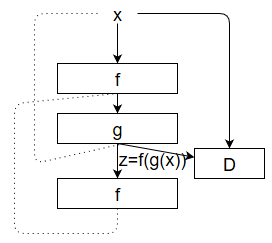
\includegraphics[width = 8 cm]{img/network.png}
	\caption{Structure of the network}
\end{figure}

The target function of the generative network $L_G=L_{GANG}+\alpha L_{CONST}+\beta L_{TID}+\gamma L_{TV}$ is a linear combination of four loss functions, each with different meanings.

\begin{itemize}
\item $L_{GANG}=\sum_{x\in \mathbf{s}}CrossEntropy(D(g(f(x))), D_t)+\sum_{x\in \mathbf{t}}CrossEntropy(D(g(f(x))), D_t)$, where $D_t$ is the result produce by the $D$ network when it is 100\% sure that the image is from the target domain. It measures the ability of the generative network to "confuse" the discriminative network, as the basic idea of GAN. 
\item $L_{CONST}=\sum_{x\in \mathbf{s}}d(f(x), f(g(f(x))))$. It means that inputs from the source domain should still have similar features after transformation.
\item $L_{TID}=\sum_{x\in \mathbf{t}}d(x, g(f(x)))$. It states that inputs from the target domain should remain identical after transformation.
\item $L_{TV}=\sum_{x\in \mathbf{s} \cup \mathbf{t}}\sum_{i,j}((z_{i+1,j}-z_{i,j})^2+(z_{i,+1j}-z_{i,j})^2)^{1/2}$, where $z=g(f(x))$ is the generated image. It ensures that the generated images does not contain too much noise.
\end{itemize}

In these formulas, $\mathbf{s}$ and $\mathbf{t}$ denote the source domain and the target domain, respectively.

\section{Experiments}

\subsection{Transforming SVHN digits into MNIST digits}

This experiment had been done in [1], and we would like to reproduce its result.

The $f$ network used in this experiment is a CNN that resembles the infamous VGGnet, but with fewer layers, as the input images are smaller and simpler. Its structure can be expressed as 64C3-64C3-P2-128C3-128C3-P2-128C3-128C3-P2-256-10, where "$x$C$y$" denotes a convolution layer with $x$ filters of size $y$, and "P2" denotes a max-pooling layer with a downsampling factor of 2. The last two layers are fully connected layers. The network is trained on the "extra" split of the SVHN dataset, which does not intersect with train and test data,to prevent training-on-test problem. It achieved an accuracy of 96.53\% on test split.

The rest of the network is mostly borrowed from [10], a Tensorflow implementation of the network used in [9], to save time from tuning GAN from scratch which is well known to be difficult. The $g$ network (the generator) is a stack of 4 deconvolution layers, and the $D$ network (the discriminator) is a stack of 4 convolution layers, which downsample by moving the convolutional filter in stride of 2, instead of the commonly used max-pooling.

To quantitatively evaluate the quality of generated images, we also trained a MNIST classifier using exactly the same structure of the $f$ network. It achieves 99.17\% accuracy on MNIST test split. It will be used to classify images generated by the GAN.

Samples of the generated images are shown in figure 2. Their quality improves as training progress, having less and less noise and glitch, although the shape of the digit do not change much. For difficult samples in SVHN, such as very blurred image or multiple digits, the corresponding generated images is likely to be awkward, not resembling any digit or even any handwritten symbol.

\begin{figure}[H]
	\centering
	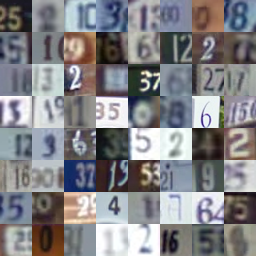
\includegraphics[width = 5 cm]{img/1000_0000_src.png}
	\\
	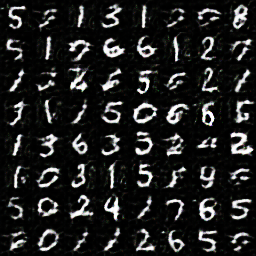
\includegraphics[width = 5 cm]{img/1000_0000_gen.png}
	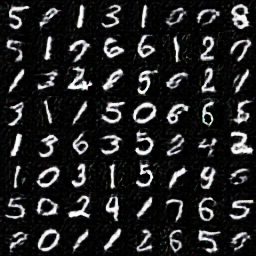
\includegraphics[width = 5 cm]{img/2000_0000_gen.png}
	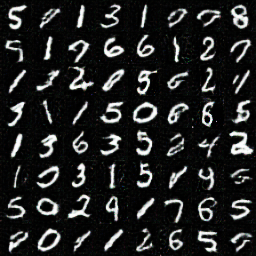
\includegraphics[width = 5 cm]{img/3000_0000_gen.png}
	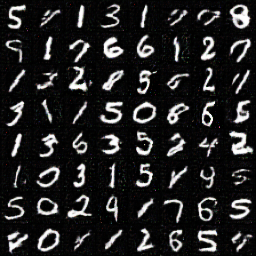
\includegraphics[width = 5 cm]{img/4000_0000_gen.png}
	\caption{Source images and generated images at 1000th (top left), 2000th(top right), 3000th(bottom left), 4000th (bottom right) iterations.}
\end{figure}

\begin{figure}[H]
	\centering
	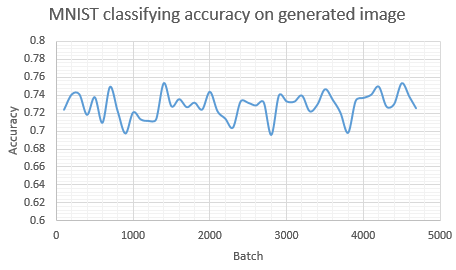
\includegraphics[width = 10 cm]{img/plot1.png}
	\caption{MNIST classifying accuracy on generated image}
\end{figure}

However, the quantitative result, namely the classifying accuracy of generated images, does not improve throughout the training, as shown in figure 3. As shown in the figure, it keeps oscillating between 70\% and 75\%. The reason may be that a robust MNIST classifier is not affected by noise or glitch in the image, but the improvement on image quality is mostly about noise and glitch. 

\subsubsection{Performance of feature extractor}

We noticed that the $f$ network used in [1] is significantly worse than one should achieve. Its test error rate, reported to be 4.95\%, is not only far worse than state-of-the-art, but also worse than many out-of-the-box model available on the Internet. [1] claimed that such performance is sufficient for the task of domain transfer, without demonstration or experiment to support the idea. We feel that validating this idea is meaningful.

To obtain networks of different performance, we simply adjust the keep rate of dropout while training it, without the need to modify its structure. Dropout with an adequate strength is commonly used to deal with overfitting, but if it is too strong, which means the keep rate is too small, the network becomes underfit, which is supposed to behave like a weaker classifier. We obtained a normal $f$ network (the one used in previous experiments) trained with a keep rate of $0.5$, and three impaired version with keep rate $0.3$, $0.2$ and $0.15$. Table 1 compares these networks. We suggest that their performances are all within the range of performances of simple CNNs that potential researchers working on this problem may use, therefore they are representative.

\begin{table}[H]
	\centering
	\caption{Comparison of normal and impaired $f$ network}
	\begin{tabular}{|l|c|c|c|c|}
	    \hline
		Keep rate & 0.5 & 0.3 & 0.2 & 0.15 \\ \hline \hline
		SVHN test accuracy & 96.53\% & 96.03\% &  94.54\% & 93.47\% \\ \hline
		Average generated image accuracy, 2000 iterations afterwards & 72.98\% & 67.29\% & 74.39\% & 68.02\% \\ \hline
	\end{tabular}
\end{table}

\begin{figure}[H]
	\centering
	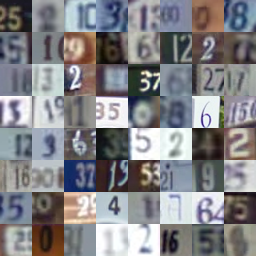
\includegraphics[width = 5 cm]{img/1000_0000_src.png}
	\\
	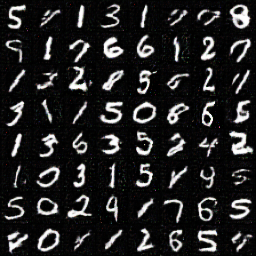
\includegraphics[width = 5 cm]{img/4000_0000_gen.png}
	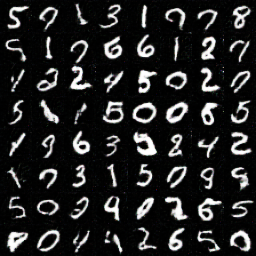
\includegraphics[width = 5 cm]{img/4000_0000_gen_D030.png}
	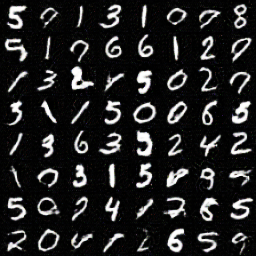
\includegraphics[width = 5 cm]{img/4000_0000_gen_D020.png}
	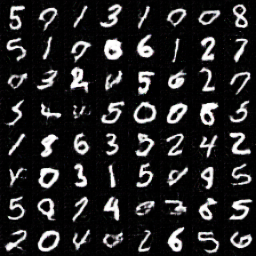
\includegraphics[width = 5 cm]{img/4000_0000_gen_D015.png}
	\caption{Source images and generated images by GANs using $f$ network trained with keep rate 0.5 (top left), 0.3 (top right), 0.2 (bottom left), 0.15 (bottom right).}
\end{figure}

\begin{figure}[H]
	\centering
	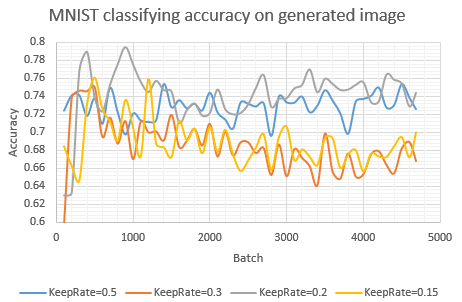
\includegraphics[width = 10 cm]{img/plot2.png}
	\caption{MNIST classifying accuracy on image generated by GANs using different $f$ networks}
\end{figure}

Qualitative and quantitative results, as shown in figure 4 and 5 respectively, shows that there is no clear and simple relationship between the quality of generated image and the performance of the $f$ network. In contrast, they varies in a seemingly random manner. The result suggest that improving the $f$ network is likely to be unnecessary for better generated images, as long as its performance is beyond modest.

\section{Conclusion}

\section*{References}

\medskip

\small

[1] Yaniv Taigman, Adam Polyak \& Lior Wolf (2016). Unsupervised Cross-domain Image Generation. ICLR 2017.

[2] Goodfellow, I., Pouget-Abadie, J., Mirza, M., Xu, B., Warde-Farley, D., Ozair, S., ... \& Bengio, Y. (2014). Generative adversarial nets. In Advances in Neural Information Processing Systems (pp. 2672-2680).

[3] Reed, S., Akata, Z., Yan, X., Logeswaran, L., Schiele, B., \& Lee, H. (2016). Generative adversarial text to image synthesis. ICML 2016.

[4] Gatys, L. A., Ecker, A. S., \& Bethge, M. (2016). Image style transfer using convolutional neural networks. In Proceedings of the IEEE Conference on Computer Vision and Pattern Recognition (pp. 2414-2423).

[5] Johnson, J., Alahi, A., \& Li, F. F. (2016). Perceptual Losses for Real-Time Style Transfer and Super-Resolution. Computer Vision – ECCV 2016. Springer International Publishing.

[6] Chen, X., Duan, Y., Houthooft, R., Schulman, J., Sutskever, I., \& Abbeel, P. (2016). Infogan: interpretable representation learning by information maximizing generative adversarial nets.

[7] Larsen, A. B. L., Sønderby, S. K., Larochelle, H., \& Winther, O. (2016). Autoencoding beyond pixels using a learned similarity metric.

[8] Odena, A., Olah, C., \& Shlens, J. (2016). Conditional image synthesis with auxiliary classifier gans.

[9] Radford, A., Metz, L., \& Chintala, S. (2015). Unsupervised representation learning with deep convolutional generative adversarial networks.

[10] https://github.com/carpedm20/DCGAN-tensorflow

\end{document}